\documentclass[11pt]{article}
\usepackage[margin=1in]{geometry}
\usepackage{fancyhdr}
\usepackage{listings}
\usepackage{graphicx}
\setlength{\parindent}{0pt}
\setlength{\parskip}{5pt plus 1pt}
\setlength{\headheight}{13.6pt}
\newcommand\question[2]{\vspace{.25in}\hrule\textbf{#1: #2}\vspace{.5em}\hrule\vspace{.10in}}

\renewcommand\part[1]{\vspace{.10in}\textbf{(#1)}}

\pagestyle{fancyplain}
\lhead{\textbf{\NAME}}
\rhead{DS - Project 3, \today}
\begin{document}\raggedright

\newcommand\NAME{Lukas Gianinazzi, Young Ban, Vincent Demotz}  % your name

\question{3}{Mini-Test}

\part{1}

\begin{itemize}
	\item Vector Clocks keep tracks of causal dependencies
	\item Vector Clocks fulfill strong clock condition
\end{itemize}

\part{2}

\begin{itemize}
\item$e^{x}_{i} \Rightarrow e^{x}_{j}$ iff $C_{i} (e^{x}_{i})[i] \leq C_{j} (e^{y}_{j})[i] \wedge 
\neg ( C_{j} (e^{y}_{j})[i] \leq C_{i} (e^{x}_{i})[i])$
\end{itemize}

\clearpage

\part{3}

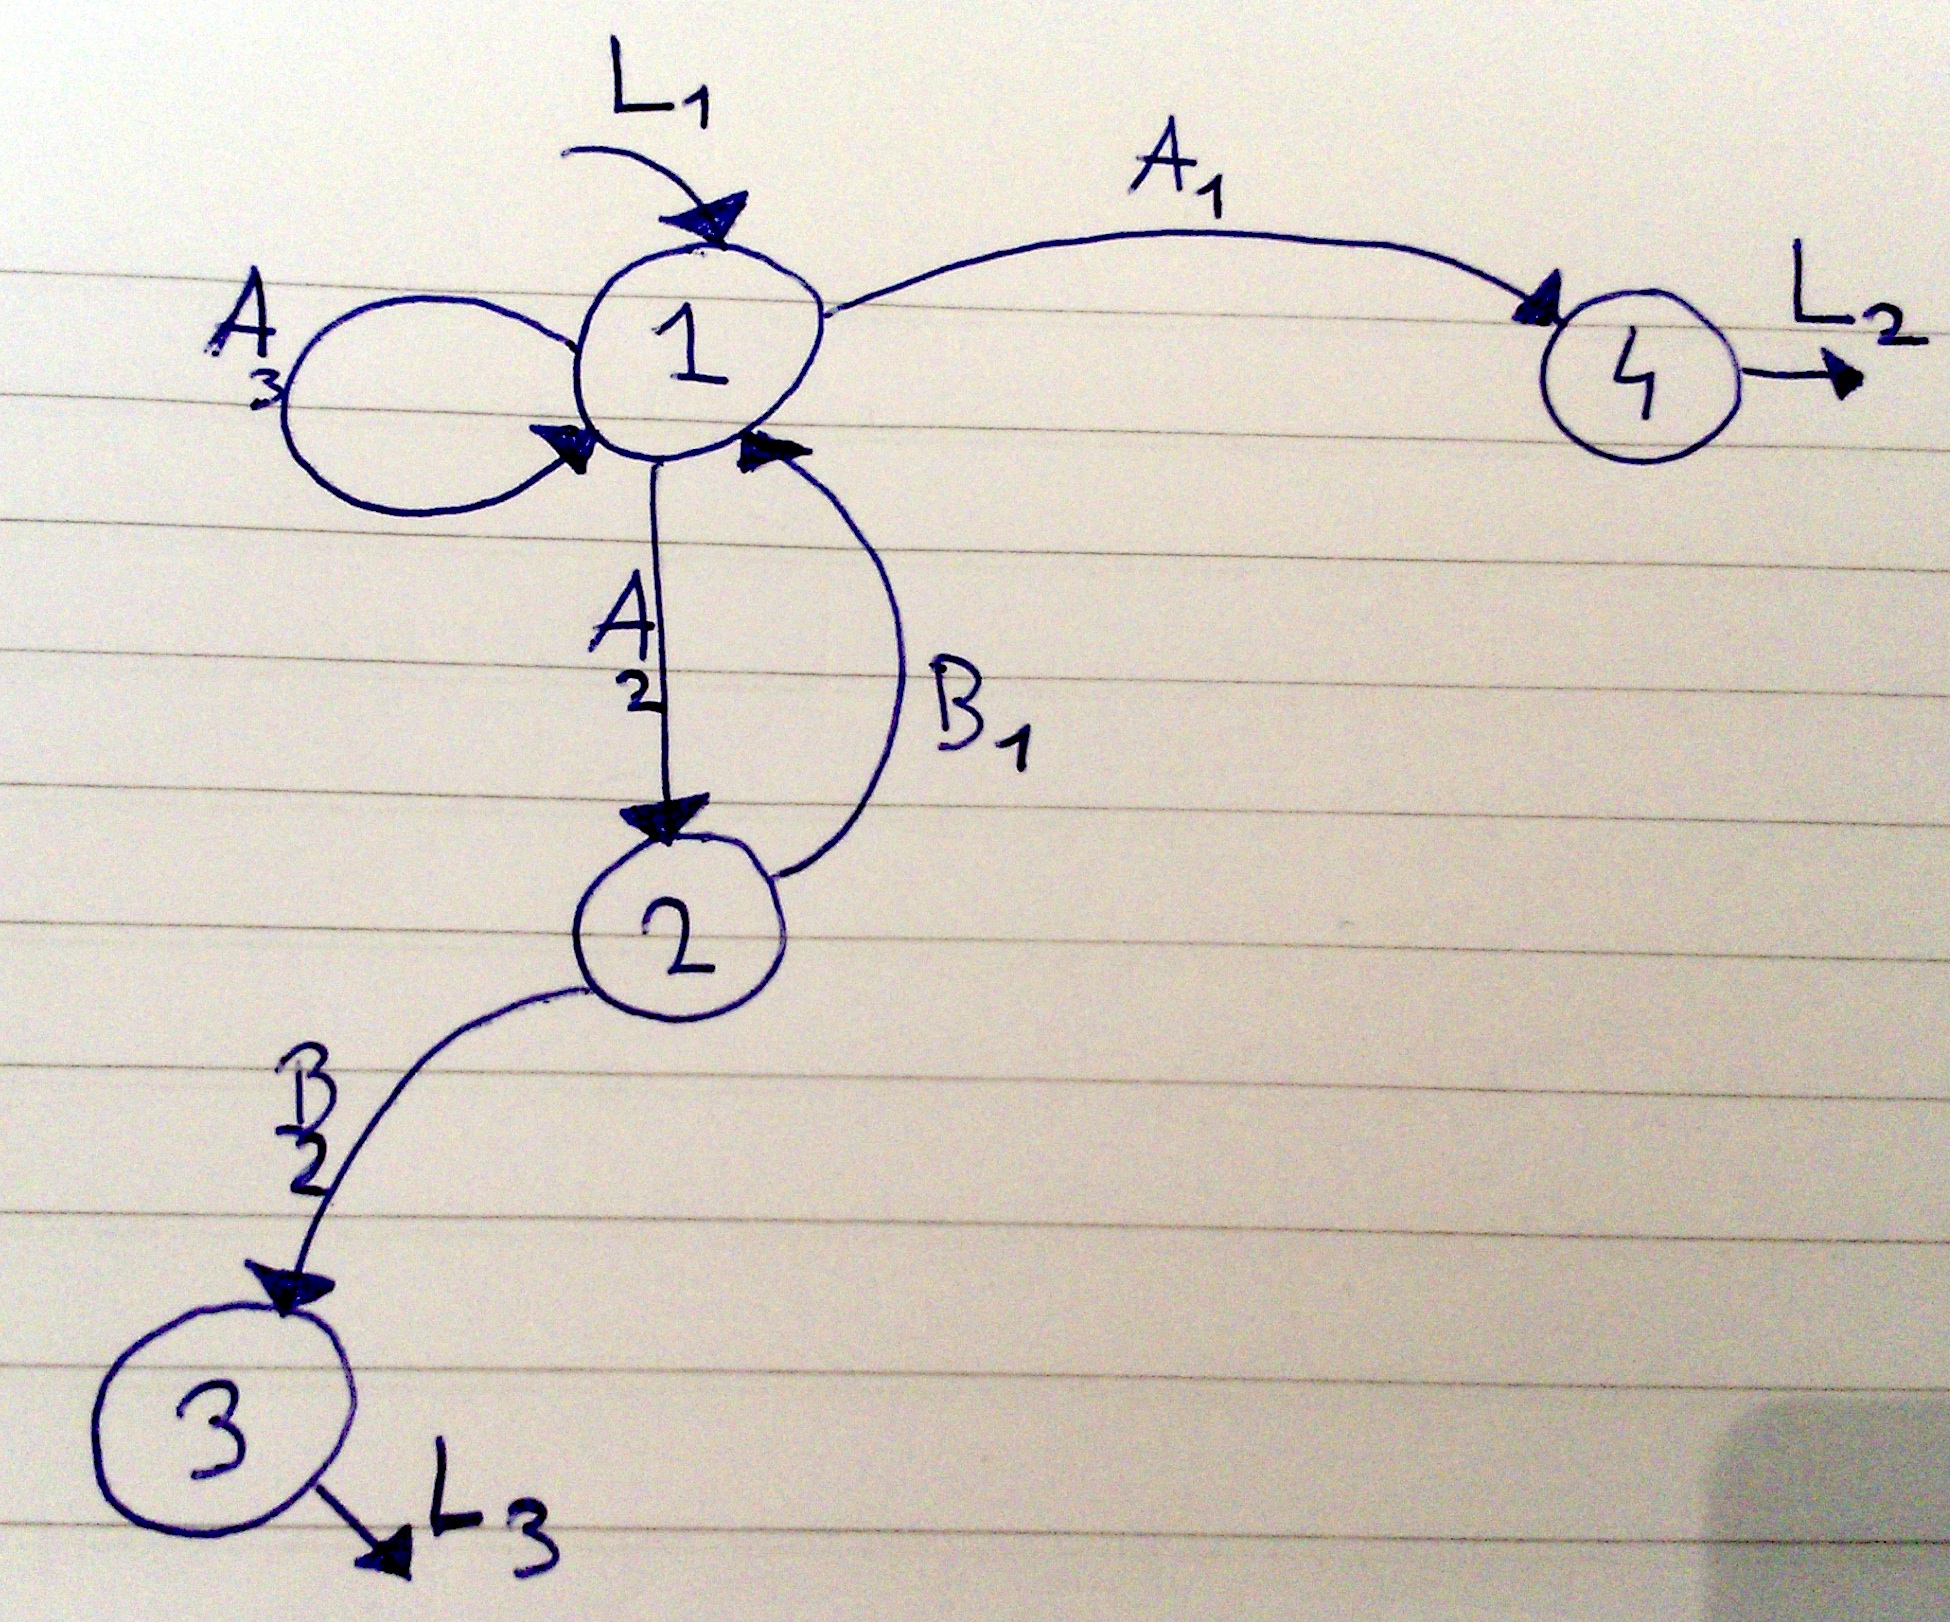
\includegraphics[scale=0.15]{registrationStates.jpg}

\textbf{Figure 1, states machine for registration}

\begin{itemize}
	\item \textbf{State 1 : } App waits for an instruction from user
	\item \textbf{State 2 : } App waits for reply from network
	\item \textbf{State 3 : } Registration succeeded, can launch MainActivity
	\item \textbf{State 4 : } App quits
	\item \textbf{$L_{1}$ : } App is launched
	\item \textbf{$L_{2}$ : } App process is destroyed
	\item \textbf{$L_{3}$ : } MainActivity is created and started
	\item \textbf{$A_{1}$ : } onBackPress() is called
	\item \textbf{$A_{2}$ : } onLogin() is called and haveNetworkConnection() returns true
	\item \textbf{$A_{3}$ : } onLogin() is called and haveNetworkConnection() returns false, display AlertDialog to inform user
	\item \textbf{$B_{1}$ : } onRegistrationFailed() is called
	\item \textbf{$B_{2}$ : } onRegistrationSucceeded() is called
\end{itemize}

\clearpage

\part{4}

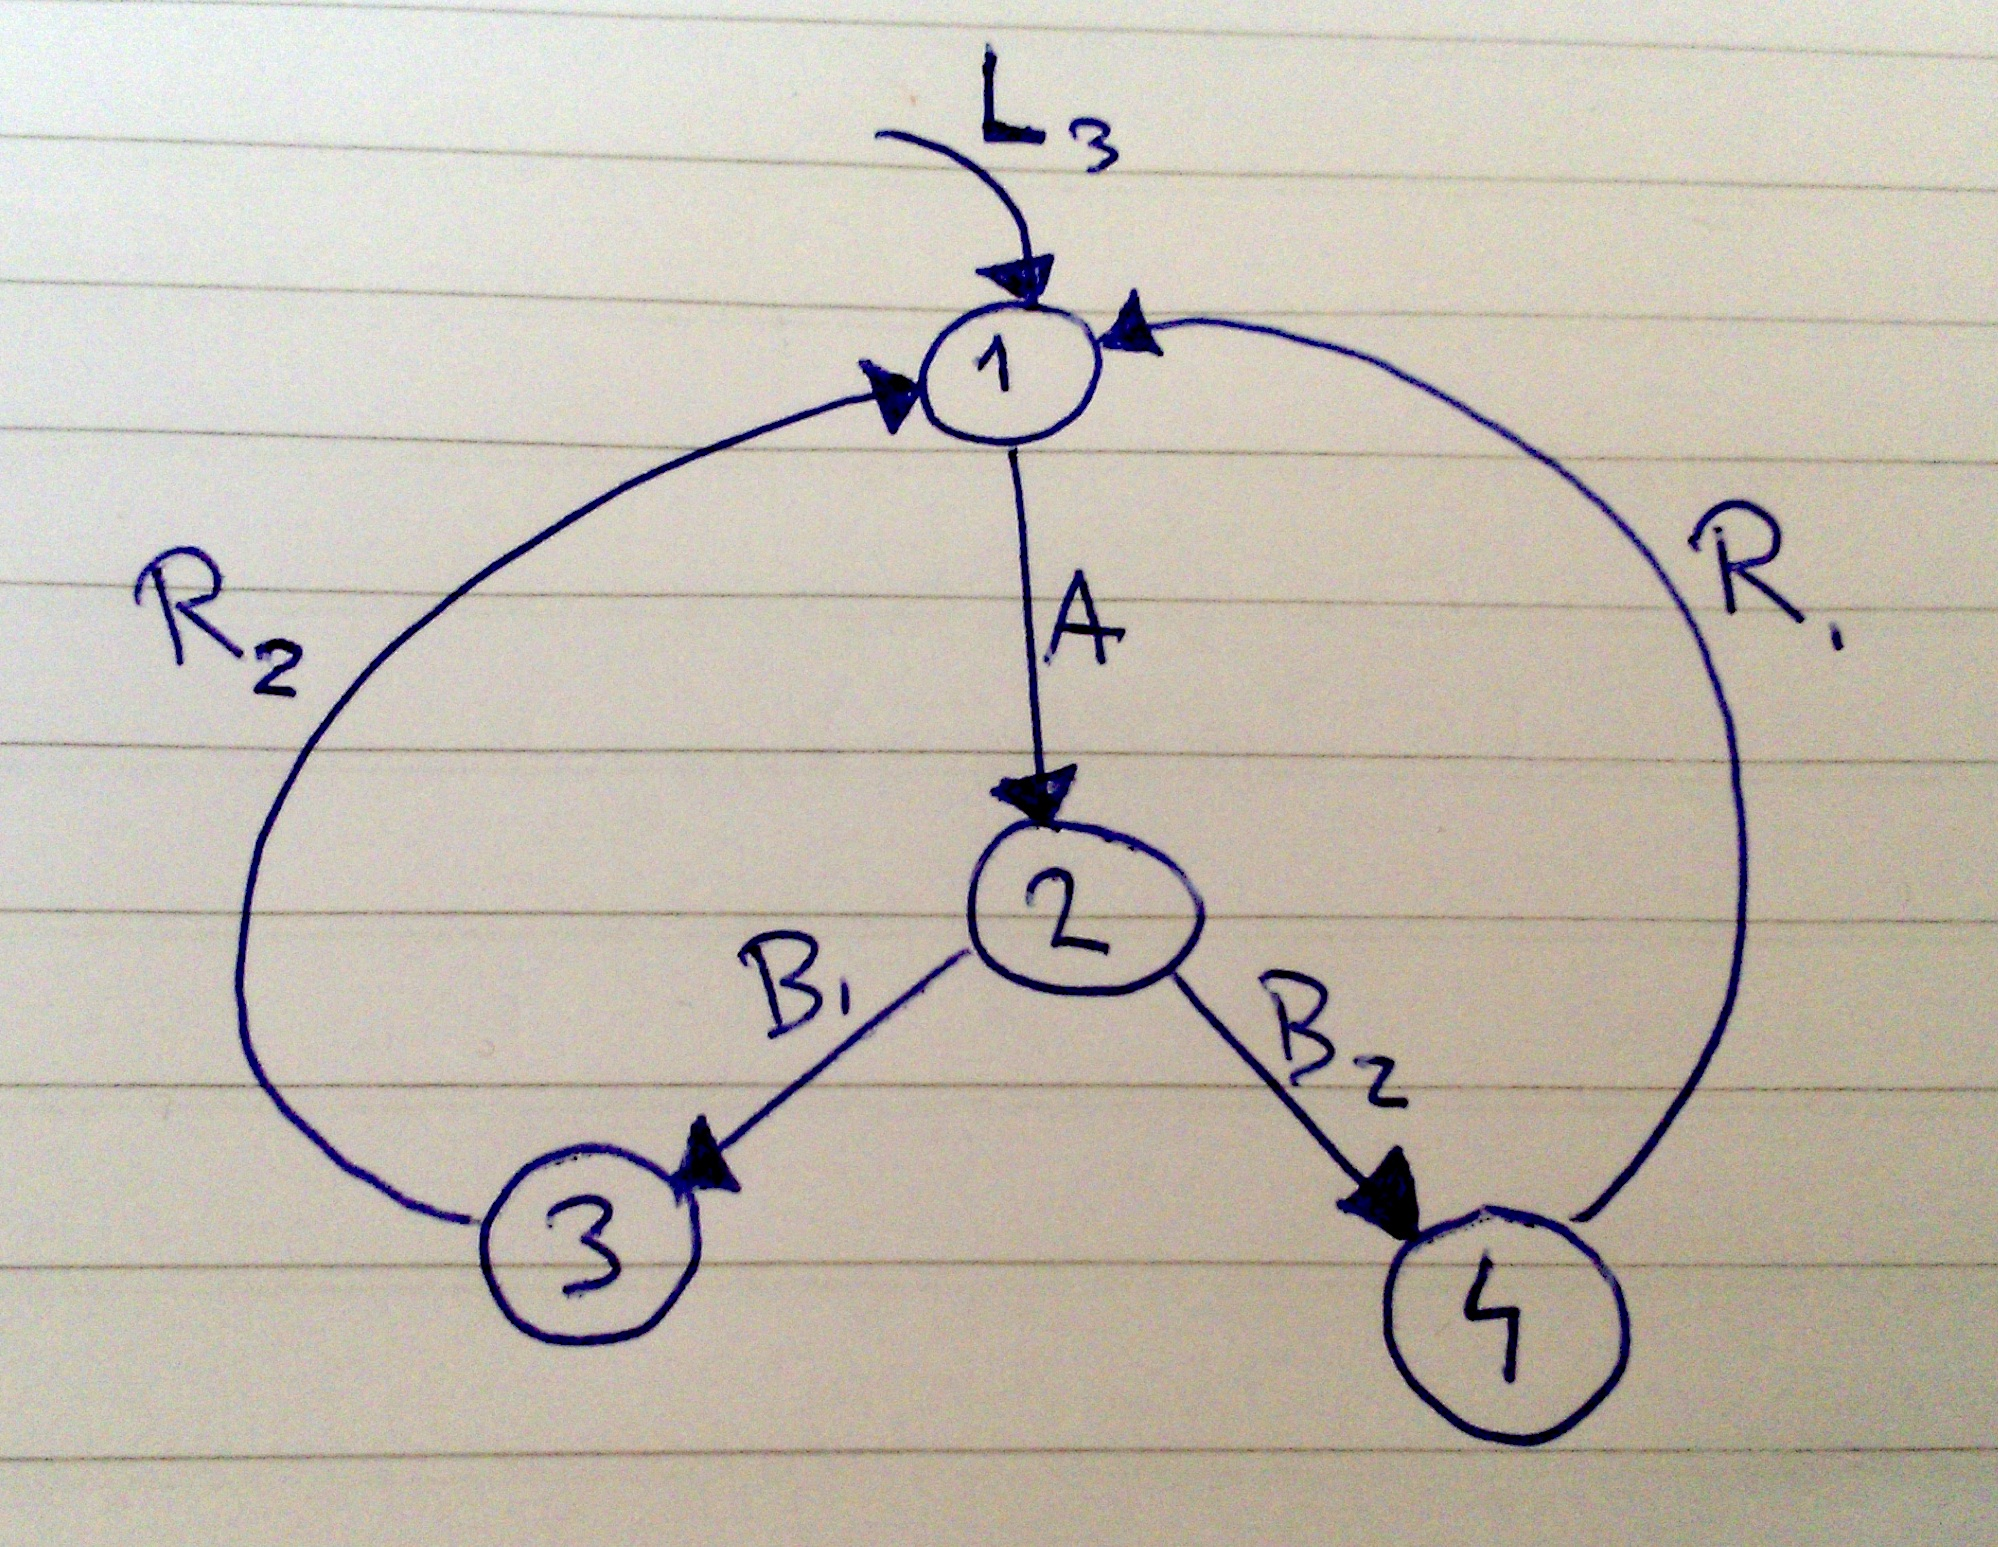
\includegraphics[scale=0.15]{sendMessageStates.jpg}

\textbf{Figure 2, states machine for send message}

\begin{itemize}
	\item \textbf{State 1 : } App waits for user to enter message
	\item \textbf{State 2 : } App waits for reply from network about the message just send
	\item \textbf{State 3 : } Message has been successfully delivered
	\item \textbf{State 4 : } Message failed to be delivered
	\item \textbf{$L_{3}$ : } User has been successfully registered
	\item A : sendMessage(String text, int id) is called on ChatLogic
	\item \textbf{$B_{1}$ : } onMessageDeliverySucceeded is called from ChatLogic
	\item \textbf{$B_{2}$ : } onMessageDeliveryFailed is called from ChatLogic
	\item \textbf{$R_{1}$ : } calls setTryToSendToFailure(int IdProvided)
	\item \textbf{$R_{2}$ : } calls setTryToSendToSend(int IdProvided)
\end{itemize}

\clearpage

\part{5}

\begin{itemize}
	\item It would be possible to sort receiving events.
\end{itemize}

\part{6}

\begin{itemize}
	\item Before. Else it would be possible to violates clock consistency condition. For example, a client A receives a message m1 with timestamps 0. Client sends a message m2 with time 0 and then tick. Clearly, we have m1 $\rightarrow$ m2 and it should imply that C(m1) $<$ C(m2), but both have timestamps 0.

\end{itemize}

\part{7}

\begin{itemize}
	\item The problem with vector clocks is that one needs to know the number of processes in advance and this number has to be fix. The paper solves the problem in proposing a solution where one has possibilities to create dynamically processes at runtime.
\end{itemize}














\end{document}